\documentclass{beamer}
\usepackage{url}
\usepackage{graphics}
\usepackage{bibunits}
\usepackage{abbrevs}
\usepackage{acronym}
\usepackage[vario]{fancyref}
\usepackage[utf8]{inputenc}
\usepackage{default}
\usepackage{gnuplot-lua-tikz}
\usepackage{multicol}

%%% BEGIN LATEX TWEAKS

% Configure bibliography
\bibliographystyle{acm}
\defaultbibliography{../references/primary}
\defaultbibliographystyle{acm}

% Acronyms for common stuff
\acrodef{aecl}[AECL]{Atomic Energy Canada Limited}
\acrodef{cgr}[CGR]{Compagnie General Radiographique}

% Abbreviation commands for common stuff
\newabbrev\ther{Therac-25}
\newabbrev\aecl{\ac{aecl}}
\newabbrev\cgr{\ac{cgr}}

%%% END LATEX TWEAKS

\title{Therac-25: Will history repeat itself?}
\author{Ash Tyndall}

\begin{document}
  \frame{\titlepage}

  \begin{frame}
  \frametitle{Table of Contents}
  \tableofcontents
  \end{frame}
  
  \section{Measuring Software-Related Failure}
  
  \begin{frame}
  \frametitle{Example Adverse Event Categories}
    \tiny
  \begin{multicols}{4}
    \begin{itemize}
  \item Failure to run on AC/DC
  \item Abnormal
  \item Absorption
  \item Accessory incompatible
  \item Measurements, inaccurate
  \item Adaptor, failure of
  \item Agglutinate, failure to
  \item Automatic injection system overinfusion
  \item Failure to back-up
  \item Failure to convert to back-up
  \item Balloon rupture
  \item Balloon asymmetrical
  \item Balloon burst
  \item Contamination during use
  \item Intermittent continuity
  \item Continuous
  \item Continuous firing
  \item Continuous mode failure
  \item Use of Incorrect Control Settings
  \item Cool, failure to
  \item Coolant, contraindicated
  \item Cooling system, failure of
  \item Insufficient cooling
  \item Display misread
  \item Erratic display
  \item No display or display failure
  \item Incorrect display
  \item Disposable
  \item Dissection
  \item Distilled water, contaminated
  \item Dome collapse
  \item Rupture due to trauma
  \item Saline, use of homemade
  \item Salt tablet(s), use of
  \item Seal, incorrect
  \item Sediment filter problems
  \item Self-activation or keying
  \item Sensing intermittently
  \item Failure to sense
  \item Inadequate training
  \item Transducer overheating
  \item Transducer probe overheating
  \item Transducer failure
  \item Transmitter failure
  \item Trocar/instrument incompatibility
  \item Tube(s), exploding of
  \item Tubing, incorrect placement of
  \item Twisting
  \item Ultrafiltration
  \item Ultraviolet
  \item Ultraviolet absorbing
  \item Uncoiled
  \item Undercorrection
  \item Warning light, incorrect
  \item Water softener process, failure of
  \item Water treatment
  \item Wedge filter problem
  \item Wedge, difficult to
  \item Screw head(s), incorrect
  \item Wavelength, incorrect
  \item Failure to zero
  \item Automatic injection system, failure to infuse
  \item Blood in tubing
  \item Metal shedding debris
  \item Electrical wires, defective
  \item Water softener regeneration cycle, mistiming of
  \item Temperature probe, loose
  \item Bubble detector, failure of
  \item Valve(s), defective
  \item Tube(s), defective
  \item Air eliminator, defective
  \item Seal, defective
  \item Cable, defective
  \item Underdelivery
  \item Electro-magnetic interference (EMI), compatibility/incompatibility
  \item Tube(s), buckling of
  \item Wire(s), breakage of
  \item Device Issue
  \item Laparoscopic sterilization
  \item Meter failure
  \end{itemize}
  \end{multicols}
  \end{frame}

  \begin{frame}
   \frametitle{Adverse Events that are ``Computer Related''}
   \smaller
   \begin{multicols}{2}
   \begin{itemize}
    \item Computer failure
    \item Computer hardware error
    \item Computer software issue
    \item Incorrect display
    \item Error or warning message, failure to produce
    \item Power calculation error due to software problem
    \item Incorrect software programming calculations
    \item Algorithms, inconsistent
    \item Semiautomatic code, failure to override
    \item Year 2000 (Y2K) related problem
    \item Date-related software issue
    \item Application network issue
    \item Application program issue
    \item Application program version or upgrade problem
    \item Application security issue
    \item Computer operating system issue
    \item Computer system security issue
    \item Data back-up problem
    \item Loss of Data
    \item Operating system becomes non-functional
    \item Operating system version or upgrade problem
    \item Problem with software installation
    \item Programming issue
   \end{itemize}
   \end{multicols}

  \end{frame}

  
  \begin{frame}
   \frametitle{Number of ``Adverse Events''}
   \begin{tikzpicture}[gnuplot]
%% generated with GNUPLOT 4.6p4 (Lua 5.1; terminal rev. 99, script rev. 100)
%% Tue 21 Oct 2014 14:08:55 WST
\tikzset{every node/.append style={font={\fontsize{9pt}{10.8pt}\selectfont}}}
\gpmonochromelines
\path (0.000,0.000) rectangle (10.922,8.128);
\gpcolor{color=gp lt color border}
\gpsetlinetype{gp lt border}
\gpsetlinewidth{1.00}
\draw[gp path] (1.411,0.886)--(1.591,0.886);
\draw[gp path] (10.422,0.886)--(10.242,0.886);
\node[gp node right] at (1.245,0.886) {1};
\draw[gp path] (1.411,1.302)--(1.501,1.302);
\draw[gp path] (10.422,1.302)--(10.332,1.302);
\draw[gp path] (1.411,1.852)--(1.501,1.852);
\draw[gp path] (10.422,1.852)--(10.332,1.852);
\draw[gp path] (1.411,2.134)--(1.501,2.134);
\draw[gp path] (10.422,2.134)--(10.332,2.134);
\draw[gp path] (1.411,2.268)--(1.591,2.268);
\draw[gp path] (10.422,2.268)--(10.242,2.268);
\node[gp node right] at (1.245,2.268) {10};
\draw[gp path] (1.411,2.684)--(1.501,2.684);
\draw[gp path] (10.422,2.684)--(10.332,2.684);
\draw[gp path] (1.411,3.234)--(1.501,3.234);
\draw[gp path] (10.422,3.234)--(10.332,3.234);
\draw[gp path] (1.411,3.516)--(1.501,3.516);
\draw[gp path] (10.422,3.516)--(10.332,3.516);
\draw[gp path] (1.411,3.650)--(1.591,3.650);
\draw[gp path] (10.422,3.650)--(10.242,3.650);
\node[gp node right] at (1.245,3.650) {100};
\draw[gp path] (1.411,4.066)--(1.501,4.066);
\draw[gp path] (10.422,4.066)--(10.332,4.066);
\draw[gp path] (1.411,4.615)--(1.501,4.615);
\draw[gp path] (10.422,4.615)--(10.332,4.615);
\draw[gp path] (1.411,4.897)--(1.501,4.897);
\draw[gp path] (10.422,4.897)--(10.332,4.897);
\draw[gp path] (1.411,5.031)--(1.591,5.031);
\draw[gp path] (10.422,5.031)--(10.242,5.031);
\node[gp node right] at (1.245,5.031) {1000};
\draw[gp path] (1.411,5.447)--(1.501,5.447);
\draw[gp path] (10.422,5.447)--(10.332,5.447);
\draw[gp path] (1.411,5.997)--(1.501,5.997);
\draw[gp path] (10.422,5.997)--(10.332,5.997);
\draw[gp path] (1.411,6.279)--(1.501,6.279);
\draw[gp path] (10.422,6.279)--(10.332,6.279);
\draw[gp path] (1.411,6.413)--(1.591,6.413);
\draw[gp path] (10.422,6.413)--(10.242,6.413);
\node[gp node right] at (1.245,6.413) {10000};
\draw[gp path] (1.411,6.829)--(1.501,6.829);
\draw[gp path] (10.422,6.829)--(10.332,6.829);
\draw[gp path] (1.411,7.379)--(1.501,7.379);
\draw[gp path] (10.422,7.379)--(10.332,7.379);
\draw[gp path] (1.411,7.661)--(1.501,7.661);
\draw[gp path] (10.422,7.661)--(10.332,7.661);
\draw[gp path] (1.411,7.795)--(1.591,7.795);
\draw[gp path] (10.422,7.795)--(10.242,7.795);
\node[gp node right] at (1.245,7.795) {100000};
\draw[gp path] (1.411,0.886)--(1.411,1.066);
\draw[gp path] (1.411,7.795)--(1.411,7.615);
\node[gp node center] at (1.411,0.609) {1994};
\draw[gp path] (2.312,0.886)--(2.312,1.066);
\draw[gp path] (2.312,7.795)--(2.312,7.615);
\node[gp node center] at (2.312,0.609) {1996};
\draw[gp path] (3.213,0.886)--(3.213,1.066);
\draw[gp path] (3.213,7.795)--(3.213,7.615);
\node[gp node center] at (3.213,0.609) {1998};
\draw[gp path] (4.114,0.886)--(4.114,1.066);
\draw[gp path] (4.114,7.795)--(4.114,7.615);
\node[gp node center] at (4.114,0.609) {2000};
\draw[gp path] (5.015,0.886)--(5.015,1.066);
\draw[gp path] (5.015,7.795)--(5.015,7.615);
\node[gp node center] at (5.015,0.609) {2002};
\draw[gp path] (5.917,0.886)--(5.917,1.066);
\draw[gp path] (5.917,7.795)--(5.917,7.615);
\node[gp node center] at (5.917,0.609) {2004};
\draw[gp path] (6.818,0.886)--(6.818,1.066);
\draw[gp path] (6.818,7.795)--(6.818,7.615);
\node[gp node center] at (6.818,0.609) {2006};
\draw[gp path] (7.719,0.886)--(7.719,1.066);
\draw[gp path] (7.719,7.795)--(7.719,7.615);
\node[gp node center] at (7.719,0.609) {2008};
\draw[gp path] (8.620,0.886)--(8.620,1.066);
\draw[gp path] (8.620,7.795)--(8.620,7.615);
\node[gp node center] at (8.620,0.609) {2010};
\draw[gp path] (9.521,0.886)--(9.521,1.066);
\draw[gp path] (9.521,7.795)--(9.521,7.615);
\node[gp node center] at (9.521,0.609) {2012};
\draw[gp path] (10.422,0.886)--(10.422,1.066);
\draw[gp path] (10.422,7.795)--(10.422,7.615);
\node[gp node center] at (10.422,0.609) {2014};
\draw[gp path] (1.411,7.795)--(1.411,0.886)--(10.422,0.886)--(10.422,7.795)--cycle;
\node[gp node center] at (5.916,0.194) {Year};
\gpcolor{color=gp lt color 0}
\gpsetlinetype{gp lt plot 0}
\draw[gp path] (1.862,1.302)--(2.312,1.718)--(3.213,1.718)--(3.664,0.886)--(4.114,1.961)%
  --(4.565,2.550)--(5.015,2.741)--(5.466,3.860)--(5.917,4.112)--(6.367,4.330)--(6.818,4.609)%
  --(7.268,4.701)--(7.719,4.901)--(8.169,5.139)--(8.620,5.251)--(9.070,5.735)--(9.521,5.898)%
  --(9.971,6.701)--(10.422,7.123);
\gpcolor{color=gp lt color border}
\gpsetlinetype{gp lt border}
\draw[gp path] (1.411,7.795)--(1.411,0.886)--(10.422,0.886)--(10.422,7.795)--cycle;
%% coordinates of the plot area
\gpdefrectangularnode{gp plot 1}{\pgfpoint{1.411cm}{0.886cm}}{\pgfpoint{10.422cm}{7.795cm}}
\end{tikzpicture}
%% gnuplot variables

  \end{frame}

  
  \begin{frame}
   \frametitle{Percentage of ``Computer Related'' Adverse Events}
   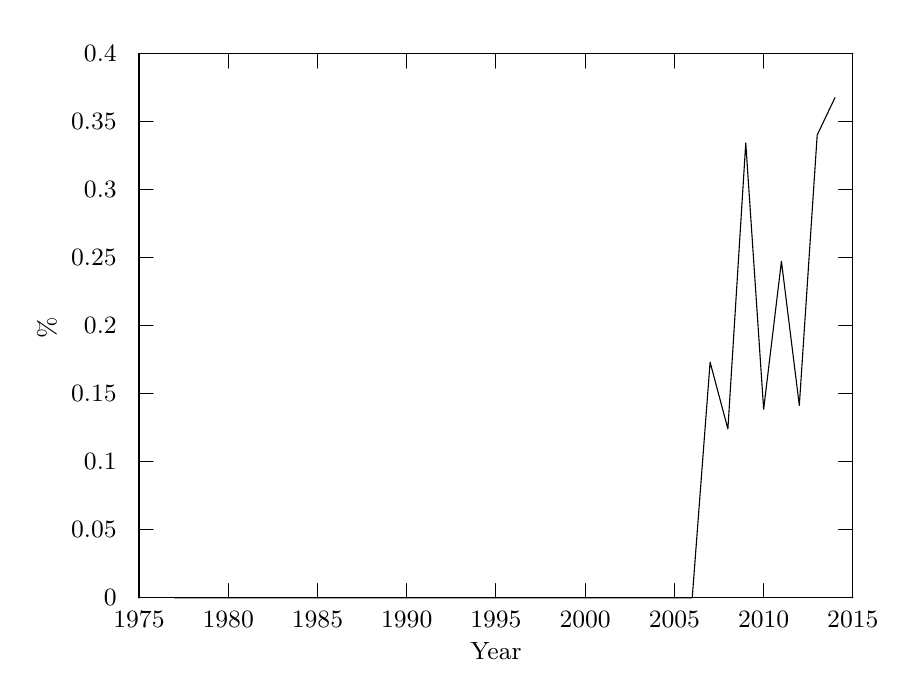
\begin{tikzpicture}[gnuplot]
%% generated with GNUPLOT 4.6p4 (Lua 5.1; terminal rev. 99, script rev. 100)
%% Wed 08 Oct 2014 21:52:41 WST
\tikzset{every node/.append style={font={\fontsize{9pt}{10.8pt}\selectfont}}}
\gpmonochromelines
\path (0.000,0.000) rectangle (10.922,8.128);
\gpcolor{color=gp lt color border}
\gpsetlinetype{gp lt border}
\gpsetlinewidth{1.00}
\draw[gp path] (1.356,0.886)--(1.536,0.886);
\draw[gp path] (10.422,0.886)--(10.242,0.886);
\node[gp node right] at (1.190,0.886) {0};
\draw[gp path] (1.356,1.750)--(1.536,1.750);
\draw[gp path] (10.422,1.750)--(10.242,1.750);
\node[gp node right] at (1.190,1.750) {0.05};
\draw[gp path] (1.356,2.613)--(1.536,2.613);
\draw[gp path] (10.422,2.613)--(10.242,2.613);
\node[gp node right] at (1.190,2.613) {0.1};
\draw[gp path] (1.356,3.477)--(1.536,3.477);
\draw[gp path] (10.422,3.477)--(10.242,3.477);
\node[gp node right] at (1.190,3.477) {0.15};
\draw[gp path] (1.356,4.341)--(1.536,4.341);
\draw[gp path] (10.422,4.341)--(10.242,4.341);
\node[gp node right] at (1.190,4.341) {0.2};
\draw[gp path] (1.356,5.204)--(1.536,5.204);
\draw[gp path] (10.422,5.204)--(10.242,5.204);
\node[gp node right] at (1.190,5.204) {0.25};
\draw[gp path] (1.356,6.068)--(1.536,6.068);
\draw[gp path] (10.422,6.068)--(10.242,6.068);
\node[gp node right] at (1.190,6.068) {0.3};
\draw[gp path] (1.356,6.931)--(1.536,6.931);
\draw[gp path] (10.422,6.931)--(10.242,6.931);
\node[gp node right] at (1.190,6.931) {0.35};
\draw[gp path] (1.356,7.795)--(1.536,7.795);
\draw[gp path] (10.422,7.795)--(10.242,7.795);
\node[gp node right] at (1.190,7.795) {0.4};
\draw[gp path] (1.356,0.886)--(1.356,1.066);
\draw[gp path] (1.356,7.795)--(1.356,7.615);
\node[gp node center] at (1.356,0.609) {1975};
\draw[gp path] (2.489,0.886)--(2.489,1.066);
\draw[gp path] (2.489,7.795)--(2.489,7.615);
\node[gp node center] at (2.489,0.609) {1980};
\draw[gp path] (3.623,0.886)--(3.623,1.066);
\draw[gp path] (3.623,7.795)--(3.623,7.615);
\node[gp node center] at (3.623,0.609) {1985};
\draw[gp path] (4.756,0.886)--(4.756,1.066);
\draw[gp path] (4.756,7.795)--(4.756,7.615);
\node[gp node center] at (4.756,0.609) {1990};
\draw[gp path] (5.889,0.886)--(5.889,1.066);
\draw[gp path] (5.889,7.795)--(5.889,7.615);
\node[gp node center] at (5.889,0.609) {1995};
\draw[gp path] (7.022,0.886)--(7.022,1.066);
\draw[gp path] (7.022,7.795)--(7.022,7.615);
\node[gp node center] at (7.022,0.609) {2000};
\draw[gp path] (8.156,0.886)--(8.156,1.066);
\draw[gp path] (8.156,7.795)--(8.156,7.615);
\node[gp node center] at (8.156,0.609) {2005};
\draw[gp path] (9.289,0.886)--(9.289,1.066);
\draw[gp path] (9.289,7.795)--(9.289,7.615);
\node[gp node center] at (9.289,0.609) {2010};
\draw[gp path] (10.422,0.886)--(10.422,1.066);
\draw[gp path] (10.422,7.795)--(10.422,7.615);
\node[gp node center] at (10.422,0.609) {2015};
\draw[gp path] (1.356,7.795)--(1.356,0.886)--(10.422,0.886)--(10.422,7.795)--cycle;
\node[gp node center,rotate=-270] at (0.221,4.340) {\%};
\node[gp node center] at (5.889,0.194) {Year};
\gpcolor{color=gp lt color 0}
\gpsetlinetype{gp lt plot 0}
\draw[gp path] (1.809,0.886)--(4.302,0.886)--(4.982,0.886)--(5.889,0.886)--(6.116,0.886)%
  --(6.569,0.886)--(6.796,0.886)--(7.022,0.886)--(7.249,0.886)--(7.476,0.886)--(7.702,0.886)%
  --(7.929,0.886)--(8.156,0.886)--(8.382,0.886)--(8.609,3.880)--(8.835,3.032)--(9.062,6.663)%
  --(9.289,3.282)--(9.515,5.161)--(9.742,3.331)--(9.969,6.764)--(10.195,7.240);
\gpcolor{color=gp lt color border}
\gpsetlinetype{gp lt border}
\draw[gp path] (1.356,7.795)--(1.356,0.886)--(10.422,0.886)--(10.422,7.795)--cycle;
%% coordinates of the plot area
\gpdefrectangularnode{gp plot 1}{\pgfpoint{1.356cm}{0.886cm}}{\pgfpoint{10.422cm}{7.795cm}}
\end{tikzpicture}
%% gnuplot variables

  \end{frame}

  \section{Bibliography}

  \begin{frame}[allowframebreaks]
    \frametitle{Bibliography}
    \tiny
    \nocite{*}
    \bibliography{primary}
  \end{frame}

\end{document}
